\chapter{Experiments}
\label{experiments:intro}

%%%%% Overview %%%%%%
In this chapter, we focus on the experiments we conducted to investigate whether and to what extent the NQM (\autoref{methods:NQM}) can be used to increase the robustness of NCAs. \autoref{Experiments:OverviewTree} gives a condensed overview for the experiments. The experiments can be divided into three blocks: First, the tests whether the NQM can be implied as a loss at all (\autoref{experiments:01.0:Into}), secondly, the construction of functioning losses (\autoref{experiments:02.0:intro}), and thirdly, the robustness tests and improvements (\autoref{experiments:03.0:Intro}). These three build on each other logically and were executed in this order. However, this is only partially the case within the sections. More often, several strands were explored simultaneously, and there are some cross-connections. These sections are organized thematically and do not build on each other chronologically or logically.\\
In \autoref{experiments:01.0:Into}, we first investigated whether the NQM could be implemented directly as a loss. This was preceded by a detailed evaluation of the existing setup, which also considered other ways of making the NQM usable. For example, by duplicating the samples for which the NQM is particularly poor in an interim evaluation. This could be done once or several times in the training cycle after a fairly large number of epochs. See also Future Works (\autoref{future_work}). However, the implementation as a loss was initially seen as the most promising solution. In \autoref{experiments:01.0:Into} we will only consider that this is technically possible in principle.\\
Subsequently, in \autoref{experiments:02.0:intro}, the goal was to develop a loss that is either better than the standard loss of the existing training setup or at least no worse. Ultimately, the latter was the case.
Finally, in \autoref{experiments:03.0:Intro} we were able to apply this loss function developed in \autoref{experiments:02.0:intro} in a simple setup on different perturbed datasets to increase robustness (\autoref{experiments:03.1.1:backbone_hippo:spike_noise}).\\
We then applied this to a more sophisticated model and dataset. However, there were fewer positive results here (\autoref{experiments:03.2.0:med_prost:intro}), so we decided to investigate the transferability further. For this purpose, we conducted experiments separately for model and dataset to narrow down the problem area (\autoref{experiments:03.3.0:med_hippo:intro_and_Augmented} and \autoref{experiments:03.4.0:backbone_prost:intro}). The results here indicate that with the approach chosen here, it is primarily the dataset that is challenging in terms of transferability and less so the model.
Furthermore, we simultaneously conducted additional tests with the successful setup (\autoref{experiments:03.1.2:backbone_hippo:pretrained}) and investigated hyperparameters (\autoref{experiments:03.1.w:Hyperpatameters}) and further loose (\autoref{experiments:03.1.x:FurtherNQMLosses}).

%%%%% Overview - Tree %%%%%%
\begin{figure}[h!]
    \centering
    \tikzstyle{selected}=[draw=red,fill=red!30]
    \tikzstyle{done}=[fill=green!45]
    \tikzstyle{tables done}=[fill=yellow!45]
    \tikzstyle{optional}=[dashed,fill=gray!50]
    \begin{tikzpicture}[dirtree]
    \node [selected] {\ref{experiments:01.0:Into} experiments}
        child { node {\ref{experiments:01.1:Only_NQM} Only NQM}}	
        child { node {\ref{experiments:02.0:intro} Dice, Bce and NQM}
            child { node {\ref{experiments:02.1:diceBce+NQM} DiceBceNQM}}
            child { node {\ref{experiments:02.2:FurtherDice-Bce-NQMLosses} Further Mixed Dice-Bce-NQM Losses}
                % child { node {\ref{experiments:02.2.1:Only_NQM_Pretrained} On Pretrained Models}}
                % child { node {\ref{experiments:02.2.2:dice+NQM} Multiplicative Dice-Bce-NQM Losses}}
            }
        }
        child { node {\ref{experiments:03.0:Intro} Robustness Improving}
            child { node {\ref{experiments:03.1.0:backbone_hippo:intro} Backbone-NCA on Hippocampus}
                child { node {\ref{experiments:03.1.1:backbone_hippo:spike_noise} Augmented Datasets}}
                child { node {\ref{experiments:03.1.2:backbone_hippo:pretrained} Pretrained Models}}
                child { node {\ref{experiments:03.1.w:Hyperpatameters} Hyperparameters}
                    child { node {\ref{experiments:03.1.3:backbone_hippo:stackSize} stacksize 2, 3, 6}}
                    child { node {\ref{experiments:03.1.4:backbone_hippo:alpha} alpha 0.5 and 2.0}}
                }
                child { node {\ref{experiments:03.1.x:FurtherNQMLosses} Non-Linear NQM Losses}
                    child { node {\ref{experiments:03.1.5:backbone_hippo:logNQM} logNQM bases 2, e, 3, 10}}
                    child { node {\ref{experiments:03.1.6:backbone_hippo:powNQM} powNQM base 3}}
                    child { node {\ref{experiments:03.1.7:backbone_hippo:sqrtNQM} sqrtNQM}}
                }
            }
            child { node {\ref{experiments:03.2.0:med_prost:intro} Med-NCA on Prostate}
                child { node {\ref{experiments:03.2.1:med_prost:augmented} Augmented Datasets}}
                child { node {\ref{experiments:03.2.2:med_prost:onDomainShifts} Domain Shifts}}
            }
            child { node {\ref{experiments:03.3.0:med_hippo:intro_and_Augmented} Med-NCA on Hippocampus}}
            child { node {\ref{experiments:03.4.0:backbone_prost:intro} Backbone-NCA on Prostate}
                child { node {\ref{experiments:03.4.1:backbone_prost:Augmented} Augmented Datasets}}
                child { node {\ref{experiments:03.4.2:Backbone_prost:DomainShifts} Domain Shifts}}
            }
        };
    \end{tikzpicture}
    \caption{Condensed overview of our experiments}
    \label{Experiments:OverviewTree}
\end{figure}

%%%%% Datasets %%%%%
\subsection*{Datasets}
\begin{figure}[h]
    \centering
        \begin{minipage}{0.49\textwidth}
        \centering
        %\includegraphics[width=0.9\textwidth]{example-image-a} % first figure itself
        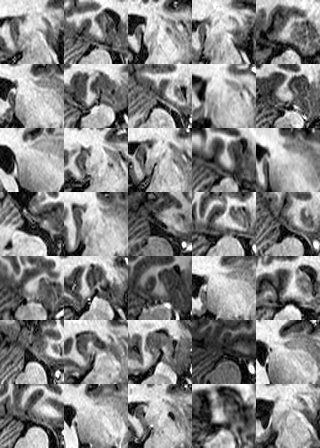
\includegraphics[width=\linewidth]{Graphics/datasets/dataset_hippo_examples_small.png}
    \end{minipage} \hfill
    \begin{minipage}{0.49\textwidth}
        \centering
        %\includegraphics[width=0.9\textwidth]{example-image-b} % second figure itself
        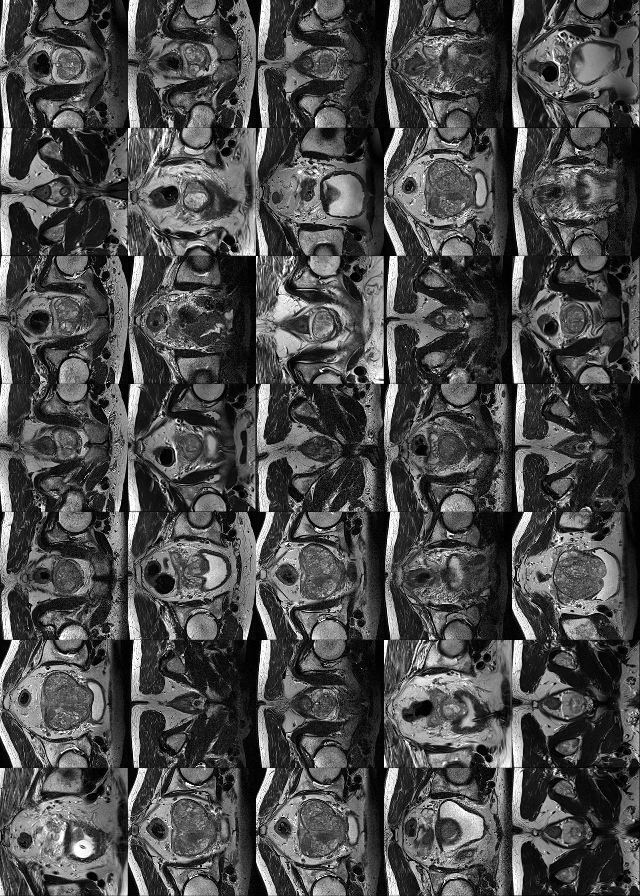
\includegraphics[width=\linewidth]{Graphics/datasets/dataset_prost_examples_small_highRes.png}
    \end{minipage}
    \caption{Example volumes from the main datasets we used. The hippocampus (left) and the prostate (right)}
    \label{fig:datasets:prost_hippo_examples}
\end{figure}

Initially, we trained mainly with the hippocampus dataset from \cite{Antonelli:2022:MedSegmentationDecatlon} and later included the prostate dataset to test transferability. The hippocampus dataset contains 394 3D volumes, and the prostate dataset has 48. We always used the train-test split of 0.7 to 0.3, indexed by \cite{Antonelli:2022:MedSegmentationDecatlon}. Some of these labels are not public. We have filtered them out. Therefor, we have 260 vital hippocampus and 26 vital prostate 3D volumes. Since these are 3D datasets, but the models we used work with 2D data, we sliced each volume. Thus, we obtained 6505 training and 2765 test 2D volumes with the hippocampus dataset and 352 training and 133 test 2D volumes with the prostate dataset. Examples can be found in \autoref{fig:datasets:prost_hippo_examples}.

\subsection*{Robustness}
\label{methods:Robust}

%%%% allgemein %%%%
In order to make robustness statements about our models (\autoref{experiments:03.0:Intro}), we generated static datasets and evaluated them continuously on the dice score. We mainly used the hippocampus and prostate datasets from the Medical Segmentation Decathlon \cite{Antonelli:2022:MedSegmentationDecatlon}. 

%%%% Augementation %%%%
We used both augmented datasets to test robustness against artifacts when they were not included in the training set and against artifacts when they were included in the training set. For the augmentations, we used the RandomSpike function and a slightly modified version of the RandomNoise function from the 'Augmentation' package of the torchIO Python library \cite{torchIO}.

%%%% DomainShifts %%%%
To test against domain shifts, we used data from 4 prostate datasets from the  
Medical Segmentation Decathlon \cite{Antonelli:2022:MedSegmentationDecatlon} (decathlon), 
parts of the UCL prostate dataset \cite{Ahmed:2017:UCL_PROMIS},
IEEE International Symposium on Biomedical Imaging \cite{Bloch:2015:ISBI_Data, Clark:2013:ISBI_TCIA} (ISBI), and the
Initiative for Collaborative Computer Vision Benchmarking \cite{Lematre:2015:i2cvb} (i2vb). We then used these to generate several domain-shifted datasets artificially. To do this, we inserted single or multiple datasets from one dataset into another, trained on them, and evaluated them on the original datasets. In addition, we generated a dataset from all prostate data available to us, trained models with different losses on it, and evaluated them on the original and training datasets.


%%%%% System %%%%%
\subsection*{System}
\label{experiments:intro:system}
We mainly trained on a system with a single NVIDIA GeForce RTX 4090, 16 AMD Ryzen 7 5700G with Radeon graphics and 58.7 GiB of main memory. The RTX 4090 has 24 GiB of VRAM, which we mostly used completely. This system was used for most tests, especially all quantitative statements and comparisons.\
Some qualitative statements are based on tests run on a other system, with seven Tesla T4, 40 Intel Xeon Silver 4210 CPU with 2.20GHz and 260GiB main memory. But there we always used only a single gpu and a single cpu. A Tesla T4 got around 16 GiB of VRAM. 


%%% --- inputs ---
\section{NQM as Lossfunction}
\label{experiments:01.0:Into}

We decided to investigate whether it is possible to include the NQM in the training loop to improve the robustness of the model by implementing the NQM directly as a loss function  or using it inside of it. To make sure that this is even possible, but also as a sensible first step in this direction, we decided to implement the NQM directly as a loss function.

In this section, we will see our first attempts to do so as a proof of concept but also to illustrate the problems that arise when using only the NQM as a loss. First, we will see in \autoref{experiments:01.1:Only_NQM} that it is technically possible to use the NQM directly as a loss function but that it has no use for training. This is because the NQM itself does not consider the label; therefore, the model will always take the opportunity to minimize the NQM as a loss by fitting into an all-one label.

%%% input %%%
%\subsection{Only NQM as a Loss}
\label{experiments:01.1:Only_NQM}
Therefore, as a first attempt at the use of the NQM for robustness, we simply defined the NQM itself as a loss:

\begin{align}
    \mathrm{NQM}\ :=\ \frac{\sum_{s\in SD} (s)} {\sum_{m\in\mu}}, \qquad
    SD = \sqrt{\frac{\sum^N_{i=1}(v_i-\mu)^2}  {N}}, \qquad
    \mu = \frac{\sum^N_{i=1}v_i}  {N}  
\end{align}

However, using this as a loss function does not work because the values below the square root in the SD and the denominator of the NQM can become zero and are then undefined.
To avoid zero-squarerooting, we choose to add an $\varepsilon$ of $e^{-8}$. To avoid zero-division, we choose to add a smoothing value of $1$. This makes the NQM loss:

\begin{align}
    \mathrm{NQM}\ :=\ \frac{\sum_{s\in SD} (s) {\color{red}+1}} {\sum_{m\in\mu} {\color{red}+1}}, \qquad
    SD = \sqrt{\frac{\sum^N_{i=1}(v_i-\mu)^2}  {N} {\color{red} + \varepsilon}}, \qquad
    \mu = \frac{\sum^N_{i=1}v_i}  {N}  
\end{align}


Loss function technically works. The model can be trained on it, but it will simply label the entire image within very few epochs since the NQM will be zero if the denominator becomes as large as possible, which is the case if the prediction is maximized. So, a model trained on this loss function will not predict anything because it will predict everything.\\
The loss function is usually a function of a model output and a label $\ell(y_i, f_\theta(x_i))$. However, since the NQM is only a function of the model output $\ell(f_\theta(x_i))$, it is not possible that a model trained on the NQM can predict anything. Therefore, it is a crude but sensible first step in exploration.


\begin{figure}[h!]
    \centering
    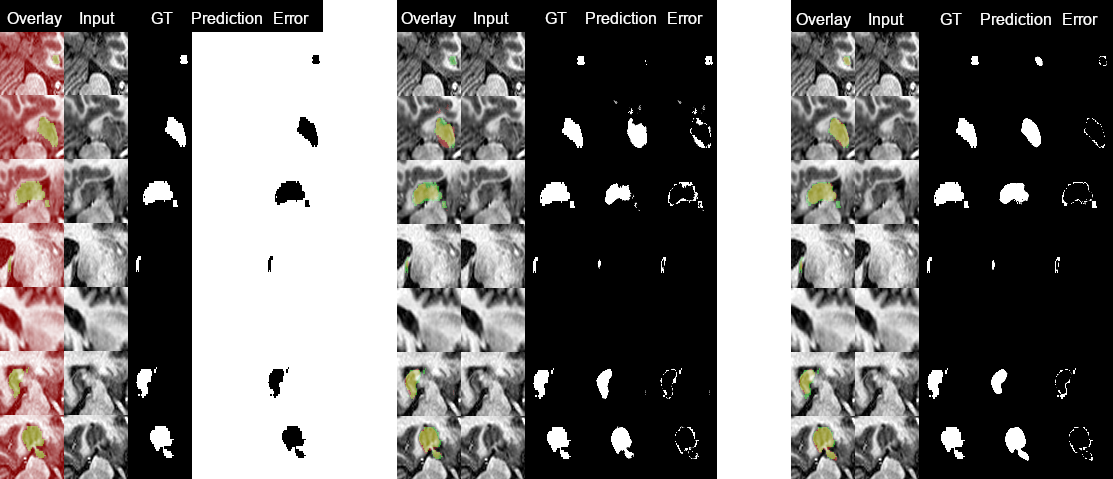
\includegraphics[width=\linewidth]{Graphics/Experiments/4.1.1_DiceBce_GT_vs._NQM_only_v2.png}
    \caption{Example image volumes (input) with ground truth labels (GT), predictions and errors. The overlay shows the input image with false positive (red), true positive (yellow), false negative (green). The model on the left was trained on the NQM as loss and clearly predicts nothing at all by simply labeling everything (overlay all red, label all white). The output stays this way from epoch 2 on. For comparison, the middle and right models were trained on DiceBCE. The middle one shows the output after 10 epochs, the right one after 500 epochs.}
    \label{fig:exp.01.1:DiceBce_vs_NQM_only}
\end{figure}           % section
\section{Dice, Bce and NQM}
\label{experiments:02.0:intro}
We decided to investigate whether it is possible to include the NQM in the training loop to improve the robustness of the model by implementing the NQM directly as a loss function or using it within the training loop. However, as seen in \autoref{experiments:01.0:Into}, it is technically possible but not very useful to use the NQM as a loss on its own. Therefore, in this section, we will focus on our attempts to implement a loss function that takes the NQM into account but not depends only on it. In \autoref{experiments:02.1:diceBce+NQM}, we will see the implementation that has worked best here, and which we have also used for most of the robustness improvement experiments (\autoref{experiments:03.0:Intro}). For completeness, the rest of this section will show some other attempts at loss functions that worked worse or not at all and that we discarded after testing them here. We also tested some other implementations not presented here, particularly those we re-tested in \autoref{experiments:03.1.x:FurtherNQMLosses}. These did not show any improvement over the DiceBceNQM loss here. They will be presented in \autoref{experiments:03.1.0:backbone_hippo:intro} for compactness.


The goal for the experiments in this section was to implement the NQM in the loss function so that the quality of the model improves or at least does not degrade. So we can build on this for robustness improvement. Therefore, we are working on the original dataset, and we used the Backbone-NCA and the Medical Segmentation Decathlon Hippocampus dataset \cite{Antonelli:2022:MedSegmentationDecatlon} and the Backbone-NCA default loss function, the DiceBCE, for comparison.


%%% --- inputs ---
\subsection{Additive Dice-Bce-NQM Loss}
\label{experiments:02.1:diceBce+NQM}
\begin{figure}[h!]
    \vspace{0.5cm}
    \centering
        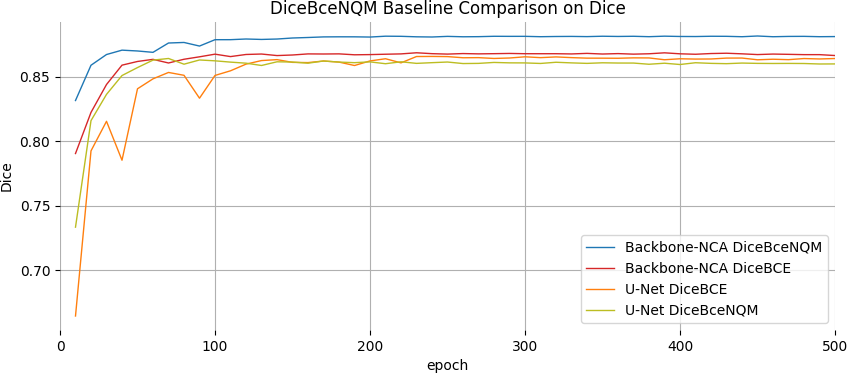
\includegraphics[width=\linewidth]{Graphics/Experiments/2.1_inverted_freeAxes_Loss_DiceLoss()_test_mask0.png}
        \caption{Backbone-NCA trained on DiceBceNQM (blue). For comparison, as baselines, a Backbone-NCA trained on DiceBCE and two U-Nets are given. The convergence of the Backbone-NCA on DiceBceNQM is quite similar to the Baselines. Therefore, training is stable on this loss regarding the Dice score. The U-Nets have been trained for 1000 epochs in total, but the Dice does not change any further, even so the train loss does.}
    \label{fig:02.1:DiceBceNQM:Baselines:onDice}
\end{figure}

As we have seen in \autoref{experiments:01.0:Into}, using only the NQM as a loss function cannot work because the reference to the ground truth label is missing, and since the models we use, the Backbone-NCA as well as the Med-NCA, already use a well working loss; the DiceBCE given in \ref{DiceBCE-Loss} is close to it, to go from there. In this way, we have developed a working NQM-loss function, which works as well as the DiceBce in our first tests, just by adding the NQM to the DiceBCE. The DiceBceNQM, as we later used it mainly for our robustness improvement experiments.

Since the NQM can be very large in the initial training cycles, we additionally cropped the NQM to a value of $\in(0,1)$ to relax the weight of the NQM in the total loss. This results in the DiceBceNQM as follows:

\begin{align}
    \text{DiceBceNQM} &:= 1 - \mathrm{Dice} + \mathrm{Bce} {\color{red}+} \mathrm{NQM},\label{eq:02.1:DiceBceNQM}\\           
    \mathrm{NQM}\ &:=\ \min\left(1, \quad \frac{\sum_{s\in SD} (s) +1} {\sum_{m\in\mu} +1}\right), \qquad
    SD = \sqrt{\frac{\sum^N_{i=1}(v_i-\mu)^2}  {N}  \varepsilon}, \qquad
    \mu = \frac{\sum^N_{i=1}v_i}  {N}               \label{eq:02.1:Only_NQM}
\end{align}

As can be seen in \autoref{fig:02.1:DiceBceNQM:Baselines:onDice} (for Dice), \autoref{fig:02.1:DiceBceNQM:Baselines:onTrainLoss} (for train losses), the Backbone-NCA converges on the DiceBceNQM about as well as on the DiceBCE, measured on Dice, or even slightly better (+1.8 points). We also trained two U-Nets, one on the DiceBCE, the other on the DiceBceNQM, as additional baselines. The convergence is approximately similar to the Backbone-NCA trained on DiceBCE. Furthermore \autoref{fig:02.1:DiceBceNQM:Baselines:Segmentations} show segmentations for the final model and baselines. As can be seen by eye the predictions with the DiceBceNQM are as good as with the DiceBCE. Putting all this together, training on this loss is stable and reliable and as least as good as on the DiceBCE alone. Therefor we used it for most of our robustness tests in \autoref{experiments:03.0:Intro}. 

\begin{figure}[h!]
    \vspace{0.5cm}
    \centering
        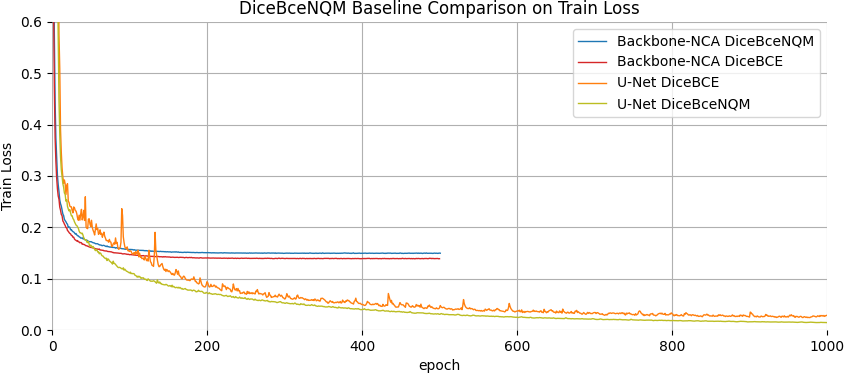
\includegraphics[width=\linewidth]{Graphics/Experiments/2.1_train_loss_freeAxes_Loss_train_0.png}
        \caption{Backbone-NCA trained on DiceBceNQM (blue). For comparison, as baselines, a Backbone-NCA trained on DiceBCE and two U-Nets are given. The convergence of the Backbone-NCA on DiceBceNQM is quite similar to the Baselines. Therefore, training is stable on this loss regarding. The U-Nets have been trained for 1000 epochs in total, Backbone-NCAs only 500 epochs.}
    \label{fig:02.1:DiceBceNQM:Baselines:onTrainLoss}
\end{figure}

\begin{figure}[h!]
    \vspace{0.5cm}
    \centering
        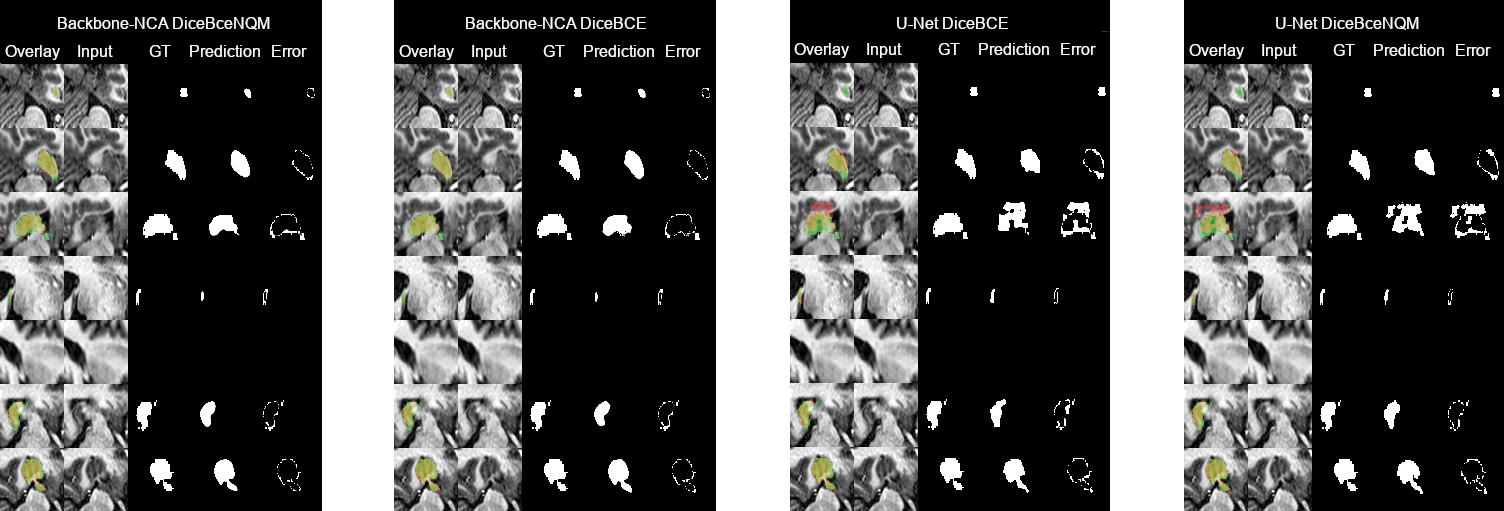
\includegraphics[width=\linewidth]{Graphics/Experiments/2.1_BaselineComparison.png}
        \caption{Backbone-NCA trained on DiceBceNQM (left). For comparison, as baselines, a Backbone-NCA trained on DiceBCE and two U-Nets are given. For each model the same image volumes (inputs) are given. With ground truth labels (GT), predictions, and errors. The overlay shows the input image with false positive (red), true positive (yellow), and  false negative (green). All for the final models after 500 epochs for Backbone-NCAs and 1000 epochs for U-Nets. First and foremost the predictions with the DiceBceNQM for the Backbone-NCA are at least as good as with the DiceBCE. Therefor training on the DiceBceNQM is stable. Even so some segmentations by the U-Nets look worse, then by the Backbone-NCAs, the Dice is is quite similar (\autoref{fig:02.1:DiceBceNQM:Baselines:onDice}).}
    \label{fig:02.1:DiceBceNQM:Baselines:Segmentations}
\end{figure}


We also tested different stacksizes and alpha-values, like in \autoref{experiments:03.1.0:backbone_hippo:intro} and here even in more configurations then there, but since, they did not show any effect here (but there), they are introduced in \autoref{experiments:03.1.0:backbone_hippo:intro}.                 % subsection
\subsection{Further Mixed Dice-Bce-NQM Losses}
\label{experiments:02.2:FurtherDice-Bce-NQMLosses}
%%%% Intro %%%% 
After and before we had our first successes with the DiceBceNQM loss (\autoref{experiments:02.1:diceBce+NQM}), in the sense that we were able to develop a loss that was no worse than the DiceBCE alone, we tried several other implementations to incorporate the NQM into the DiceBCE loss. However, they were all worse than the DiceBceNQM, or at least no better. However, since the DiceBceNQM was the simplest of the equally good losses, we decided, in the spirit of Occam's razor, to start the robustness experiments (\autoref{experiments:03.0:Intro}) with the DiceBceNQM. The more promising of these were tested again in \autoref{experiments:03.1.x:FurtherNQMLosses}, but showed no improvement over the DiceBceNQM in the experiments here without robustness testing, and were judged here to be more computationally expensive or were developed later and are therefore not yet available. These losses are presented in \autoref{experiments:03.1.x:FurtherNQMLosses} and are omitted here to avoid duplication, even though they are clearly better. For the sake of completeness, we list here the loss functions that are worth mentioning, even if they did not make it to the next round.

For the case of the additive DiceBceNQM (\autoref{experiments:02.1:diceBce+NQM}), we also tested whether taking only Dice+NQM or only Bce+NQM had a positive effect, but as suspected, this was not the case.


%%%% Offen / TODO %%%%
\iffalse
... hier stimmte irgendwas nicht ...
... diceBceMasks (Bce with no reduction) was used and the nqm was put in as weight, before the mean was build ... therefore the nqm was calculated pixelwise ... but did not work
\begin{align}
    \mathrm{DiceBceMaskNQM}     &= \mathrm{DiceLoss} + \mathrm{mean} (NQM_mask \cdot \mathrm{BCE})\\
    \mathrm{BCE}(x,y)           &=  -[y_n \cdot \log x_n + (1-y_n) \cdot \log (1-x_n)]\\
    \mathrm{DiceLoss}           &= 1 - \frac{2 \cdot {\sum^D(y \cdot f_\theta(x))}}
                                            {\sum^D(f_\theta(x)) + \sum^D(f_\theta(x))}
\end{align}
... diceBce SD
... Bce weighted with NQM


\fi
%%%% Inputs %%%%
\paragraph{NQM Loss on Pretrained Model}
\label{experiments:02.2.1:Only_NQM_Pretrained}
As a first "naive" test to circumvent the problems in \autoref{experiments:01.1:Only_NQM}, before we developed the DiceBceNQM (\autoref{experiments:02.1:diceBce+NQM}), we have taken a pretrained models with the DiceBCE.

\begin{align}
    \ell(y_i, f_\theta(x_i))\ :=
      \begin{cases}
        \mathrm{DiceBCE} & \text{if epoch {\color{red}$\leq n$}}\\
        \mathrm{NQM} & \text{else}\\
      \end{cases}
\end{align}

Regardless of how long the model was pretrained, as soon as the loss was switched to the NQM the loss dropped enormously quickly towards zero, for the same reason, as for the NQM alone. The output looks the same as in \autoref{fig:exp.01.1:DiceBce_vs_NQM_only} (left).

%%% Alternating
Since it is only a little adjustment form there, we also checked, if this can already be prevented if we alternate between the NQM and DiceBCE. So the loss becomes:

\begin{align}
    \ell(y_i, f_\theta(x_i))\ :=
      \begin{cases}
        \mathrm{NQM} & \text{if epoch {\color{red} mod $x=0$}}\\
        \mathrm{DiceBce} & \text{else}\\
      \end{cases}
\end{align}

However, this attempt suffers from the same problem. For comparison, \autoref{fig:exp.02.1:alternating} shows that already after three epochs on the NQM, the output looks as bad as \autoref{experiments:01.1:Only_NQM} and moreover, already in the very first epoch no useful prediction is left anymore So, for larger $x$ this attempt only takes longer but still converges to the same state, while the epochs with the DiceBCE work in the opposite direction.

\begin{figure}[h!]
    \centering
    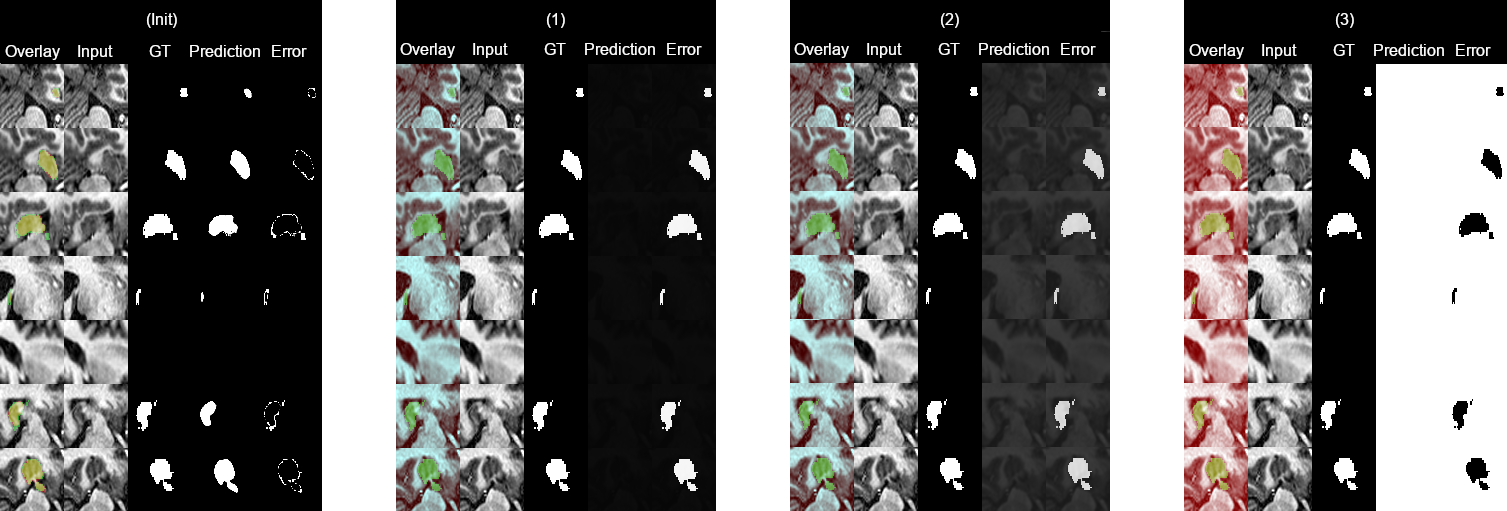
\includegraphics[width=\linewidth]{Graphics/Experiments/4.2.1_Alternating_3epochs_v3.png}
    \caption{Image samples volumes (inputs) with ground truth labels (GT), predictions, and errors. The overlay shows the input image with false positive (red), true positive (yellow), and  false negative (green). From left to right: The initial state, pretrained on DiceBCE (Init), the three very first epochs of training on the NQM.}
    \label{fig:exp.02.1:alternating}
\end{figure}
\paragraph{Multiplicative Dice-Bce-NQM Losses}
\label{experiments:02.2.2:dice+NQM}
To give the NQM more weight in the loss, we also used the NQM as a factor before the DiceBCE. Therefore, we tested the following three implementations of a multiplicative DiceBceNQM loss. However, they all suffered from the same problem as the NQM alone (\autoref{experiments:01.1:Only_NQM}) and the pretrained versions (\autoref{experiments:02.2.1:Only_NQM_Pretrained}). DiceBce*NQM-2 and 3 canceled only the part that has been multiplied with the NQM. Therefore, we tested, with the NQM as defined in \autoref{eq:02.1:Only_NQM}:

\begin{align}
    \text{DiceBce*NQM-1}\ &:=\ {\color{red}\mathrm{NQM}\ \cdot\ }(1 - \mathrm{Dice} + \mathrm{Bce})\\
    \text{DiceBce*NQM-2}\ &:=\ {\color{red}\mathrm{NQM}\ \cdot\ }(1 - \mathrm{Dice}) + \mathrm{Bce}\\
    \text{DiceBce*NQM-3}\ &:=\ 1 - \mathrm{Dice} + {\color{red}\mathrm{NQM}\ \cdot\ }\mathrm{Bce}\\ 
\end{align} % subsection                   % section
\section{Robustness Improving}
\label{experiments:03.0:Intro}
\begin{figure}[h!]
    \centering
    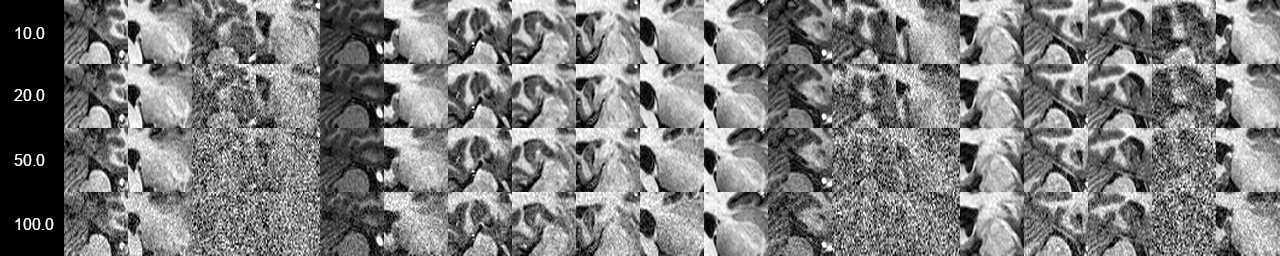
\includegraphics[width=\linewidth]{Graphics/datasets/datasets_hippo_randNoise_v2.png}\\
    \vspace{5pt}
    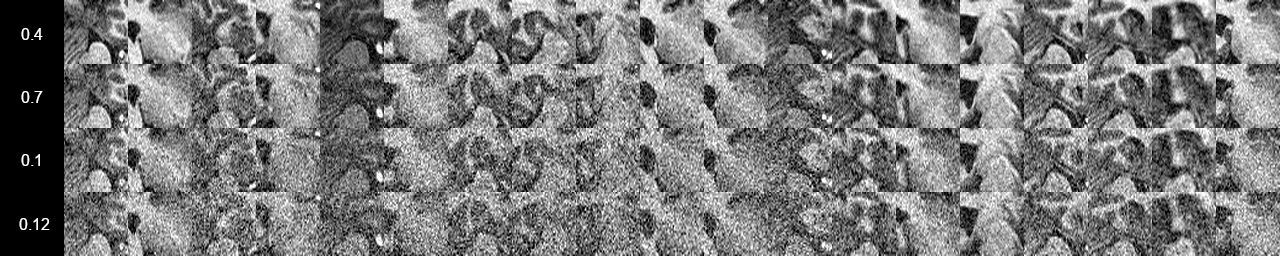
\includegraphics[width=\linewidth]{Graphics/datasets/datasets_hippo_normNoise_v2.png}
    \caption{Different noise functions that we tried for augmentation on the hippocampus dataset \cite{Antonelli:2022:MedSegmentationDecatlon}. The Standard deviation of the Gaussian distribution from which the noise is sampled is given on the very left. Top 4: Random noise function from torchIO \cite{torchIO}. As can be seen, the same images are always strongly affected. Bottom 4: Our simple addition to the random noise function with additional max-normalization, which we used for our test runs. As can be seen, the noise is much more evenly distributed across different images. Bottom 4: From top to bottom with increasing standard deviation in the noise function.}
    \label{fig:augemented:datasets:noise_problem}
\end{figure}

%%%% Allgemein Intro %%%%
Since in \autoref{experiments:01.1:Only_NQM} some adaptations of the DiceBCE loss with the NQM, all in front of the DiceBceNQM (\autoref{eq:02.1:DiceBceNQM}), no performance degradation could be seen, but also no improvement over the original data, we performed corresponding dedicated robustness tests. These are presented in this section.

Since \cite{kalkhof:2023:M3D-NCA} has already used the NQM to test the performance of models on augmented datasets in order to make robustness statements about the models, it is close to test, whether the DiceBceNQM improves robustness on a model, trained on perturbed data. To do this, we artificially perturb datasets. On the one hand with artificial augmentations to simulate different types of radiological image noise, on the other hand by adding individual data volumes from other datasets to our primary dataset to simulate data shifts.\\
As datasets, we mainly used the hippocampus and prostate datasets from the Medical Segmentation Decathlon \cite{Antonelli:2022:MedSegmentationDecatlon}. For the data shift, others accordingly (see below).

%%%% Augmentation %%%% 
For the augmentations, we statically generated four series of 5 perturbed datasets and the original dataset so that all models are trained on the same data. We used the hippocampus and prostate datasets from \autocite{Antonelli:2022:MedSegmentationDecatlon}. The datasets we generated are composed as follows and were selected according to the following criteria \begin{itemize}
    \item A series of 5 augmented datasets, each for the hippocampus and the prostate dataset, enriched with different proportions of spike artifacts.
    In each case, the goal was to decrease the dice performance of our GT model by 30 percentage points when all data were augmented ("Spike 1.0"). The four other datasets were then spiked with the same intensity, but only 0.3, 0.2, 0.1, and 0.01 shares of the data. We used the random spike function from the TorchIO package \autocite{torchIO}.
    We refer to these datasets as "Spike 1.0", "Spike 0.3", "Spike 0.2", "Spike 0.1", and "Spike 0.01", respectively. 
    \item A series of 5 augmented datasets, each on the hippocampus and the prostate dataset, using the same procedure but with random noise. We used an adapted variant of the random noise function from the TorchIO package \autocite{torchIO}. We have extended it with a simple max-normalization so that the noise is distributed much more homogeneously across the different images of the dataset, and the noise function can still be used together with the other functions of the package. The difference can be seen in \autoref{fig:augmented:datasets:noise_problem}. The problem was that in the hippocampus dataset, the max-value for the volumes varies a lot, and the standard noise function does not normalize for this.
    We refer to these datasets as "Noise 1.0", "Noise 0.3", "Noise 0.2", "Noise 0.1", and "Noise 0.01", respectively.
\end{itemize}

%%%% DomainShifts %%%%
For the domain shifts, we used data from 4 prostate datasets from the  
Medical Segmentation Decathlon \cite{Antonelli:2022:MedSegmentationDecatlon} (decathlon, decath), which we used as the main dataset. We inserted parts of other datasets into this dataset. Namely, parts of the prostate dataset from the PROMIS study \cite{Ahmed:2017:UCL_PROMIS} (ucl), the
IEEE International Symposium on Biomedical Imaging prostate dataset \cite{Bloch:2015:ISBI_Data, Clark:2013:ISBI_TCIA} (isbi), and the
Initiative for Collaborative Computer Vision Benchmarking Prostate dataset \cite{Lematre:2015:i2cvb} (i2vb). Here, we have generated a total of 2 series of datasets:\begin{itemize}
    \item A series of the decathlon dataset and 3 "shift" datasets, where we have added a sample from another dataset to the decathlon dataset. We call these "decath," "shift 1 isbi," "shift 1 i2cvb," and "shift 1 ucl," respectively.
    \item A series of the decathlon dataset and 3 "shift" datasets, where we added several samples from another dataset to the decathlon dataset because no or little change was seen in the shift 1 datasets. In each case, we aimed for a drop of about 15 points on the dice score. This dropped at very different rates, so we added four samples for ucl (dice drop 13.6), eight samples for i2cb (dice drop 15.8), and 12 samples for isbi (dice drop 16.7).
    We call this "decath," "shift 12 isbi," "shift 8 i2cvb," and "shift 4 ucl," respectively.
    \item As well as one dataset from all our available samples. We call this "all joined".
\end{itemize}

%%%% Beides %%%%
To get as broad a picture as possible, we trained at least one series for each variation of our loss functions that we tested, both for the augmentations and domain shifts. For each series that we tested, we always trained one model for each dataset, creating cohorts of models. As ground truth, we trained a cohort for each series on the standard loss function of the models we used, the DiceBCE \autoref{methods:NCA}. We constantly evaluated the Dice score on all datasets of the series (\autoref{Tables}). For the domain shifts, we also tested on all original datasets (decath, isbi, i2cb, ucl) and the all joined datasets. To do this, we had to split the tables.


%%%% Chapter Übersicht %%%%
We first explored if robustness changes occur on augmented data, with the Backbone-NCA and the hippocampus dataset with augmentations, and performed the most extensive variation of experiments on this constellation (\autoref{experiments:03.1.0:backbone_hippo:intro}). After the first positive results regarding robustness on augmented data, we checked whether this could be transferred to another model, the Med-NCA, and another dataset, the prostate dataset, as well as domain shifts (\autoref{experiments:03.2.0:med_prost:intro}). Since the results here were somewhat mixed, we decided also to examine the transfers individually. So we tested a different model, the Med-NCA, on the same dataset (\autoref{experiments:03.3.0:med_hippo:intro_and_Augmented}), as well as the same model but on a different dataset (\autoref{experiments:03.4.0:backbone_prost:intro}).
But, when using the Med-NCA on the hippocampus dataset, there is no difference at all between DiceBCE and DiceBceNQM. When using the Backbone-NCA from the prostate dataset, the results for augmentations and domain shifts were very similar to those obtained using the Med-NCA. There was only a difference in the all joined dataset, where the DiceBceNQM performed worse with the Backbone-NCA than the DiceBCE, while it performed better with the Med-NCA. In our opinion, this is also the most interesting point to pursue the DiceBceNQM further when using combined datasets with the already very powerful Med-NCA.

\begin{figure}[h!]
    \centering
    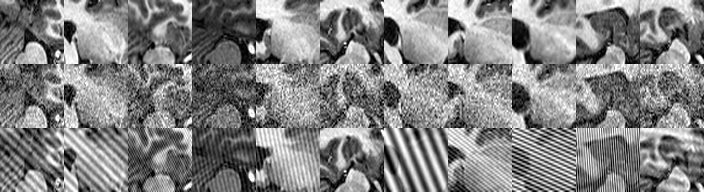
\includegraphics[width=\linewidth]{Graphics/datasets/datasets_hippo_augmented.png}\\
    \vspace{5pt}
    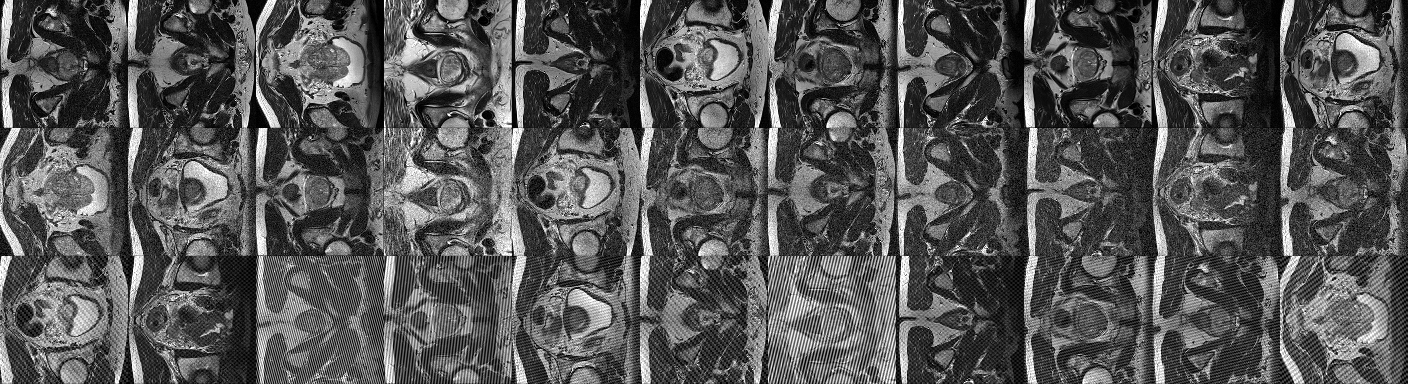
\includegraphics[width=\linewidth]{Graphics/datasets/datasets_prostate_all_augmented_highRes.png}
    \caption{Top 3: Examples from the hippocampus dataset we used. Bottom 3: Examples from the prostate datasets we used. For each 3: from top to bottom: Original from \autocite{Antonelli:2022:MedSegmentationDecatlon}, augmented with noise, augmented with spikes. We used the same noise and spike functions as here for the other datasets we generated for our test series, where only parts were augmented. However, we used different noise and spike functions for the hippocampus and prostate, as we wanted to achieve a sufficient drop in performance for our ground truth model.}
    \label{fig:augemented:datasets:augemented_hippo_prostate}
\end{figure}

%%% --- inputs ---
\subsection{Backbone-NCA on Hippocampus}
\label{experiments:03.1.0:backbone_hippo:intro}
In this section, we come to our most commonly used setup and the most comprehensive results. 
As first setup for the robustness test, we choose the BackboneNCA (\autoref{methods:NCA:Models}) and the hippocampus dataset with spike and random noise augmentations as they have just been presented.

First, we will see in \autoref{experiments:03.1.1:backbone_hippo:spike_noise} that the DiceBceNQM improves the robustness to radiological noise compared to the DiceBCE 
by up to 7 points on the Dice when artifacts were sparse (''0.01'') in the dataset, and by up to 15 points on the Dice when no artifacts were present in the training dataset, and also leads to no degradation in all other tests in this setup.

In the subsequent parts, we present several approaches to improve this setup further. Of particular note are the speedup achieved by using pretrained models (\autoref{experiments:03.1.2:backbone_hippo:pretrained}) and a minimum stacksize of 2 (\autoref{experiments:03.1.3:backbone_hippo:stackSize}). With both approaches, we did not notice any loss of robustness gain due to the DiceBceNQM.

Then we introduce the hyperparameter alpha ($\alpha$) in \autoref{experiments:03.1.4:backbone_hippo:alpha}, which at a value of 2.0 increases robustness furthermore compared to DiceBceNQM without alpha by up to 4 points on the Dice.
Finally, in \autoref{experiments:03.1.x:FurtherNQMLosses} we come to the testing of alternative nonlinear loss functions with NQM, where especially the sqrtNQM (\autoref{experiments:03.1.7:backbone_hippo:sqrtNQM}) is a promising candidate, mainly because this loss shows equivalent robustness improvements, but should converge faster. However, speed tests in this regard were not part of this work.

%%% --- inputs ---
\subsubsection{Augmented Datasets}
\label{experiments:03.1.1:backbone_hippo:spike_noise}
To test how the DiceBceNQM (\autoref{experiments:02.1:diceBce+NQM}) performs on augmented data, we trained one model with the DiceBceNQM and one model with the DiceBCE for each spike and noise dataset, as well as the original dataset without augmentations. A total of 22 models. The results can be seen in \autoref{tab:03.1.1:DiceBCE+NQM_vs_DiceBCE_on_Noise} and \autoref{tab:03.1.1:DiceBCE+NQM_vs_DiceBCE_on_Spike}. We tested these models on all datasets of the series (i.e., all Spike or all Noise datasets as well as the original dataset). The models trained on the DiceBCE for each dataset serve as a baseline for the models trained on the DiceBceNQM. The test results of DiceBceNQM - Spike 1.0 are compared to the test results of DiceBCE - Spike 1.0, the test results of DiceBceNQM - Noise 1.0 are compared to the test results of DiceBCE - Noise 1.0, and so on. The models with DiceBceNQM perform significantly better than the models with DiceBCE alone. All models are better or no worse. The range goes from -1 to +15 on the Dice and is massively positive, and almost all values are positive. Also noteworthy are the vast improvements on the fully augmented data (Noise 1.0 and Spike 1.0) of the models trained on the original dataset, for Spike +9 points, for Noise +15, as well as the vast improvements for the Spike models trained on the sparsely augmented data (Spike 0.01) of +7 points on Spike. Noise has ''only'' +2 points here.

Therefore, using the DiceBceNQM improves robustness in this setting without adverse effects. First and foremost, a model trained with DiceBceNQM on the original dataset becomes much more robust on both spiked and noisy datasets than if trained with DiceBCE alone. Furthermore, the models trained on sparse augmented datasets (Spike 0.01 and Noise 0.01), as well as all others, also benefit from the DiceBceNQM, or at least are not degraded by it.

\input{content/experiments/03_Robustness_Improving/03.1_Backbone_and_Hippocampus/tables/table_03.1.1_Aug_spike_noise}
\iffalse
\begin{table}%[h!]
    \centering
    \begin{tabular}{|c|l|l|l|l|l|}
        \hline
        \bfseries dataset serie & mean on signed & mean on absolute & sum & sum on absolute & range\\\hline
        % ---
        Spikes & 0.0092 & 0.0103 & 0.331 & 0.371 & (-0.009, +0.087) \\\hline
        Noise  & 0.0092 & 0.0097 & 0.331 & 0.351 & (-0.003, +0.154)\\\hline
        % ---
    \end{tabular}
    \caption{Aggregations over the improvements$(+)$ and deteriorations$(-)$, using the DiceBceNQM compared to the DiceBCE on Dice. All values of the experiments used for theses Aggregations: \autoref{tab:03.1.1:DiceBCE+NQM_vs_DiceBCE_on_Spike} and \autoref{tab:03.1.1:DiceBCE+NQM_vs_DiceBCE_on_Noise}}
    \label{tab:03.1.1:Aug_Spike_Noise_Aggregated}
\end{table}
\fi
\subsubsection{Pretraind Models}
\label{experiments:03.1.2:backbone_hippo:pretrained}
\begin{figure}[h!]
    \centering
        \begin{minipage}{0.49\textwidth}
        \centering
        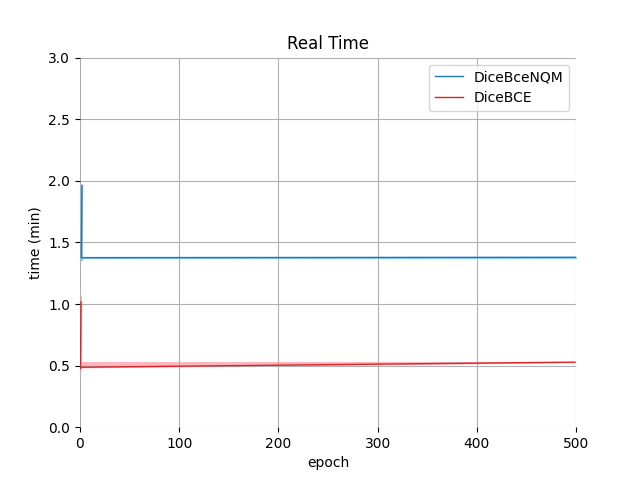
\includegraphics[width=\linewidth]{Graphics/Experiments/3.1.2_realTime_with_error_.png}
    \end{minipage} \hfill
    \begin{minipage}{0.49\textwidth}
        \centering
        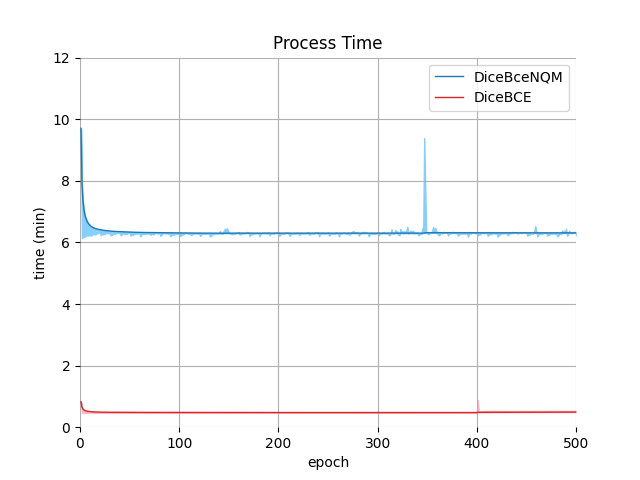
\includegraphics[width=\linewidth]{Graphics/Experiments/3.1.2_process_time_with_errors_.png}
    \end{minipage}
        \caption{Speed comparison between DiceBce and DiceBceNQM for real-time and process time. The average training times per epoch are shown in dark colors. The difference to the actual training times is shown in light colors behind the average. The DiceBceNQM takes much longer to train. The overall means for the real-time are 1.38 min and 0.49 min. The mean values for the process time are 6.33 min and 0.48 min.}
    \label{fig:DiceBCE+NQM:Pretrained:Speedcompare}
\end{figure}

Training on the DiceBceNQM with a stack size of 3 takes about 13.19 times as long as training on the DiceBCE alone and about 2.8 times as long in real time on the system we used (\autoref{experiments:intro:system}, as can be seen in \autoref{fig:DiceBCE+NQM:Pretrained:Speedcompare}). This is simply because with the stacksize, the number of predictions that need to be generated for the NQM is many times greater than without it. We mostly used a stacksize of 3 in our experiments. Therefore, we tested whether we could perform similarly by using pretrained models. To do this, we first trained a cohort of models on the Spike Hippocampus and not augmented datasets. Half of the cohort was trained for the entire 600 epochs on DiceBceNQM. The other half was pretrained for 500 epochs on DiceBCE and another 100 epochs on DiceBceNQM. The results are given in \autoref{tab:3.1.2:DiceBCE+NQM:Pretrained}. The pretrained models are continuously approximately as good as those fully trained on the DiceBceNQM. This is true for the models trained on augmented datasets and those trained on not augmented datasets. The one trained on the non-augmented dataset tends to get a little worse, but compared to the one trained on only 500 epochs \autoref{tab:03.1.1:DiceBCE+NQM_vs_DiceBCE_on_Spike}, both are better on the spike datasets and similar as good on the non-augmented one. Especially for those trained on the sparsely augmented dataset (Spike 0.01), the pretrained performs better rather than worse. 

The equivalence of these training methods is further emphasized when we look at the accumulations of the differences between pretrained and fully trained models for the entire cohort we trained for Dice: The maximum delta was $+ 0.037$, the sum of deltas was $-0.002$, the mean of the absolute deltas was $0.007$, the mean of signed deltas between these two groups was smaller in amount than $0.001$, up to these levels of accuracy. Each for the differences between the two models from the different groups trained on the same datasets (as shown as $\pm$ in the table).
\input{content/experiments/03_Robustness_Improving/03.1_Backbone_and_Hippocampus/tables/table_03.1.2_pretrained}
\subsubsection{Hyperparameters}
\label{experiments:03.1.w:Hyperpatameters}

%%% was 03.1.3
\paragraph{stackSize}   
\label{experiments:03.1.3:backbone_hippo:stackSize}

In our experiments so far, we have used a \textit{stacksize} ($N$) of 3 for the DiceBceNQM, as defined in \autoref{eq:02.1:DiceBceNQM}. This seemed sufficient so far since different stack sizes had no effect when tested on not augmented data only \autoref{experiments:02.0:intro}. We want to test if these results also hold for augmented data. Nevertheless, training with the DiceBceNQM and a stacksize of 3 already takes about 2.8 times the real-time and 13.19 times the process time compared to the DiceBCE (\autoref{fig:DiceBCE+NQM:Pretrained:Speedcompare}). We trained a cohort of models on a stacksize of 6 but only on 3 spike datasets. We had to reduce the batch size to 16 because there was not enough VRAM for that large stacksize. Therefore, the models with a stacksize of 3, which we used for comparison, are also trained with a batch size of 16. The results can be seen in \autoref{tab:3.1.3:higherStacksize}. As one can see, there is no positive or negative effect of increasing the stacksize.

Since increasing the stacksize had no effect, we also tested whether a stacksize of 2 would be sufficient and, therefore, cheaper in terms of computation. This experiment was done later on a pretrained model with the stacksize we used elsewhere. As seen in \autoref{tab:3.1.3:smallerStacksize}, it does not worsen the results. Therefore, a stacksize of 2 can be considered sufficient or better, especially concerning the non-enlarged dataset. Unfortunately, this experiment was carried out very late, so our other experiments are still done on stacksize 3.
% Aggregated values are given in \autoref{tab:3.1.3:stackSize_aggregated}
\iftable
\input{content/experiments/03_Robustness_Improving/03.1_Backbone_and_Hippocampus/tables/table_03.1.3_stackSize}
\fi

%%% alpha was 03.1.4  %%%
\paragraph{alpha}   
\label{experiments:03.1.4:backbone_hippo:alpha}
Here, we have checked whether it makes a difference if the proportion of the NQM in the total DiceBceNQM is varied. To do this, we added the parameter alpha ($\alpha$) so that the previous DiceBceNQM corresponds to $\alpha=1.0$, i.e:

\begin{align}
    \text{DiceBce-$\alpha$NQM} &:= 1 - \mathrm{Dice} + \mathrm{Bce} + {\color{red}\alpha}\cdot\mathrm{NQM}
\end{align}

Where the NQM is defined as in \autoref{eq:02.1:Only_NQM}. We have trained two cohorts. One with halved and one with doubled $\alpha$. We trained all models for 100 epochs each on a pretrained model, as in \autoref{experiments:03.1.2:backbone_hippo:pretrained}. The results in \autoref{tab:3.1.4:alpha} shows that a double $\alpha$ further increases the robustness. This is especially true when training on the less augmented dataset, and there is no degradation when training on not augmented data.

Beyond these variations on the same loss function with different alphas, we tested other loss functions that should converge more strongly and penalize higher NQM values more strongly. We will look at this in the following.
\iffalse
\input{content/experiments/03_Robustness_Improving/03.1_Backbone_and_Hippocampus/tables/table_03.1.4_alphas}
\fi
\subsubsection{Non-Linear NQM Losses}
\label{experiments:03.1.x:FurtherNQMLosses}
\begin{figure}[h!]
    \centering
        \begin{minipage}{0.49\textwidth}
        \centering
        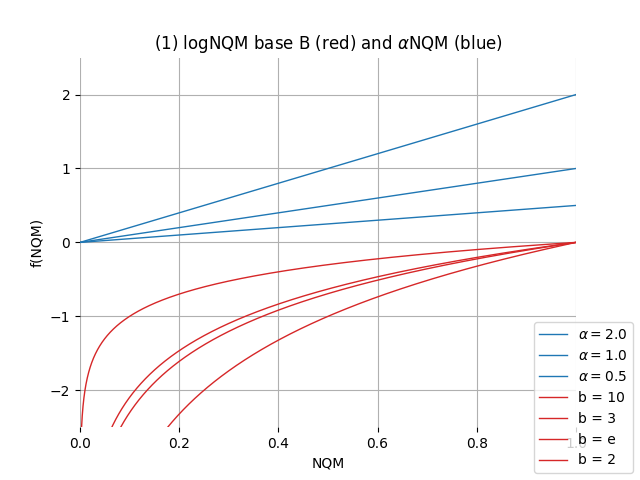
\includegraphics[width=\linewidth]{Graphics/Experiments/3.1_alphas_logs.png}
    \end{minipage} \hfill
    \begin{minipage}{0.49\textwidth}
        \centering
        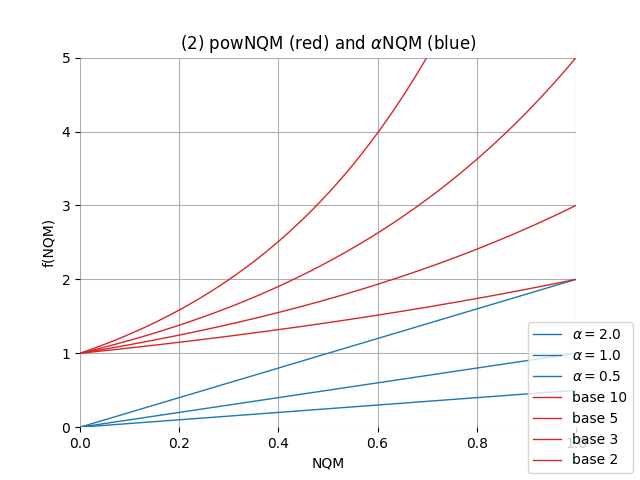
\includegraphics[width=\linewidth]{Graphics/Experiments/3.1_alphas_pow.png}
    \end{minipage}
    \begin{minipage}{0.49\textwidth}
        \centering
        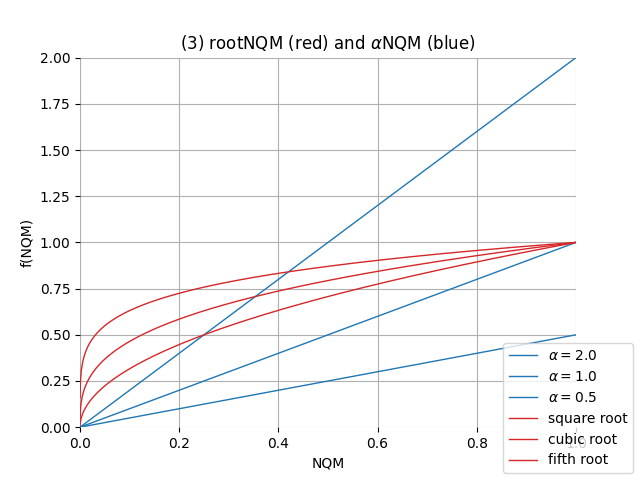
\includegraphics[width=\linewidth]{Graphics/Experiments/3.1_alphas_root.png}
    \end{minipage}
    \caption{Non-linear functions we used for NQM losses (red), to test, if they perform similar or better in comparison to the linar DiceBce-$\alpha$NQM (blue). The order in the legend within a color also corresponds to the order in which the functions are superimposed in the plot. In the range of the NQM $(0, 1)$.}
    \label{fig:furtherFunctionsForNQM}
\end{figure}

Since we have seen promising results with the linear NQM alone and with different alphas in terms of robustness to augmented data, we decided to test whether other loss functions with NQM could lead to similar or even better results. On the one hand, we chose functions that might converge more strongly because they weight higher NQM values more strongly than linear functions (logarithm, power, and root functions) or might converge similarly well. Examples of these can be seen in \autoref{fig:furtherFunctionsForNQM}. Each is compared to the linear case for the three slopes we tested in \autoref{experiments:03.1.4:backbone_hippo:alpha} (blue). 

For our experiments here, we used a pretrained model that we first trained for 500 epochs on the DiceBCE. Then, we trained this model for another 100 epochs on the corresponding loss.
We trained a cohort for each loss to be tested. Each cohort was trained on the original and with spikes augmented hippocampus datasets because this is where we have seen the clearest results with the DiceBceNQM so far. So, there are six datasets in total and one model for each dataset in each cohort. For the comparisons here, we assumed the DiceBceNQM, i.e., corresponding to $\alpha=1.0$, and trained one cohort accordingly.

%%% log NQM %%%
\paragraph{Logarithmic NQM Loss}
\label{experiments:03.1.5:backbone_hippo:logNQM}
Since the NQM assumes a value between 0 and 1, and the logarithm (log) falls to 0 faster than linearly, particularly small values are rewarded very highly with the log, i.e., the total loss is greatly reduced. This means that the NQM's share of the total loss is no longer capped (unlike in the other cases). Since this negative growth occurs at different rates with different bases, we tested several log functions with different bases. Therefore, the logNQM base B is defined as:

\begin{align}
    \text{logNQM base B} &:= 1 - \mathrm{Dice} + \mathrm{Bce} + {\color{red}\log_B}\mathrm{NQM}
\end{align}

We decided to test bases 2, e, 3, and 10. So, we trained a total of 4 cohorts on the logNQM. As seen in \autoref{tab:3.1.5:logNQM}, using a logarithmic NQM leads to mixed results compared to the linear NQM. In particular, on the original dataset, the logNQM consistently leads to a degradation of up to 9 points on the dice. On the other hand, when training on the augmented dataset, the logNQM results in a slight improvement of up to 3 points. \autoref{tab:3.1.5:logNQM_aggregated} shows various aggregations of the improvements and deteriorations in scores for each cohort. Again, there is an overall almost neutral but negative mean on the signed differences and a range shift clearly into the negative.\\\
Our implementation of the NQM with this loss could not further improve the robustness. 
% \todo{evt. Fehler bei den Labels zeigen, die mit höherer Base schlimmer werden ... war hier relativ klar zu sehen, bei manchen samples ... dann Verknüpfung nach onlyNQM, weil vermutlich ähnlihcer grund ... wobei hier der Dice immernoch über die 100 epochen gefallen ist.}
\iftable
\input{content/experiments/03_Robustness_Improving/03.1_Backbone_and_Hippocampus/tables/table_03.1.6_powNQM}
\fi

\begin{table}[h!]
    \centering
    \begin{tabular}{|c|l|l|l|l|}
        \hline
        \bfseries logNQM base & mean on signed & mean on absolute & sum on absolute & range\\\hline
        % ---
        2   & -0.0004 & 0.0063 & 0.226 & ( -0.053, +0.030)\\
        e   & -0.0011 & 0.0076 & 0.275 & ( -0.038, +0.033)\\
        3   & -0.0031 & 0.0074 & 0.266 & ( -0.086, +0.014)\\
        10  & -0.0011 & 0.0056 & 0.2   & ( -0.037, +0.024)\\\hline
        % ---
    \end{tabular}
    \caption{Aggregations over the improvements$(+)$ and deteriorations$(-)$, using the logNQM losses compared to the DiceBceNQM on Dice. All values of the experiments used for this Aggregations: \autoref{tab:3.1.5:logNQM}}
    \label{tab:3.1.5:logNQM_aggregated}
\end{table}


%%% pow NQM %%%
\paragraph{Power NQM Loss}
\label{experiments:03.1.6:backbone_hippo:powNQM}
As one can see in \autoref{fig:furtherFunctionsForNQM}, the power function is the opposite of the log function. While the log function rewards particularly small values in the range $(0,1)$ more, the power function punishes exceptionally high values. We have implemented this loss due to the range of the NQM in $(0,1)$ by choosing a constant base and placing the NQM in the exponent. Conversely, when using the NQM to the pow of something, growth is slower than linear in this interval.
Therefore, the powNQM base is defined as B:

\begin{align}
    \text{powNQM base B} &:= 1 - \mathrm{Dice} + \mathrm{Bce} + {\color{red} \mathrm{B}}^\mathrm{NQM}
\end{align}

Here, we have trained a cohort on base 3. The results are shown in \autoref{tab:3.1.6:powNQM}. The aggregated improvements and degradations are given in \autoref{tab:3.1.6:powNQM_aggregated}. As can be seen, the powNQM hardly leads to any change, which is evident when looking at the corresponding base function in \autoref{experiments:03.1.x:FurtherNQMLosses}, since the pow function with base 3 behaves almost linearly here. However, the tendency here is similar to logNQM, that models trained on the not augmented data perform worse on the augmented data. The reverse does not seem to be the case.
Therefore, it might be interesting to test a higher base again, but this was not done in the context of this work \autoref{future_work}.

\begin{table}[h!]
    \centering
    \begin{tabular}{|c|l|l|l|l|}
        \hline
        \bfseries pow NQM base & mean on signed & mean on absolute & sum on absolute & range\\\hline
        % ---
        3 & -0.0008 & 0.0073 & 0.263 & (-0.046, +0.024)\\\hline
        % ---
    \end{tabular}
    \caption{Agreggations over the improvements$(+)$ and deteriorations$(-)$, using the powNQM compared to the DiceBceNQM on Dice. All values of the experiments used for theses Aggregations: \autoref{tab:3.1.6:powNQM}}
    \label{tab:3.1.6:powNQM_aggregated}
\end{table}

\iftable
\input{content/experiments/03_Robustness_Improving/03.1_Backbone_and_Hippocampus/tables/table_03.1.5_logNQM}
\fi

%%% sqrt NQM %%%
\paragraph{Square Root NQM Loss}
\label{experiments:03.1.7:backbone_hippo:sqrtNQM}
As seen in \autoref{fig:furtherFunctionsForNQM}, the root function in the interval $(0,1)$ decays to zero, similarly to the logarithmic function. However, they do not try to reach $-\infty$ but fall to zero. This means that very small values in the root functions have very little weight. At the same time, there is a low upper bound of one that the function can assume. That way, the NQM's share of the total loss is limited, in contrast to the logarithmic function in particular, which has no limit at all, but also to the power functions, where the upper bound corresponds to the base and grows accordingly. We tested the square root function since this shows the described behavior most clearly. 
Therefore, the sqrtNQM is defined as:

\begin{align}
    \text{sqrtNQM} &:= 1 - \mathrm{Dice} + \mathrm{Bce} + \sqrtRed{\text{NQM}} 
\end{align}

Again, we trained a cohort on this loss. The results are shown in \autoref{tab:3.1.7:sqrtNQM}. The aggregated improvements and deteriorations are shown in \autoref{tab:3.1.7:sqrtNQM_aggregated}. Again, there does not appear to be much difference from the linear implementation. There may be a slight improvement in the minimally augmented dataset (spike 0.01). At the same time, there is no degradation in the not augmented dataset. This is different for logNQM and powNQM. This makes the sqrtNQM a candidate for speeding up the approach. Further experiments with domain shifts and other datasets would be interesting, too. Possibly also as cubic root or a mixture of pow and root function, in the sense of powNQM -1 + sqrtNQN (\autoref{future_work}). 

\begin{table}[h!]
    \centering
    \begin{tabular}{|c|l|l|l|l|}
        \hline
        \bfseries sqrt NQM & mean on signed & mean on absolute & sum on absolute & range\\\hline
        % ---
        & -0.0023 & 0.0084 & 0.304 & (-0.026, +0.033)\\\hline
        % ---
    \end{tabular}
    \caption{Agreggations over the improvements$(+)$ and deteriorations$(-)$, using the sqrtNQM compared to the DiceBceNQM on Dice. All values of the experiments used for theese Aggregations: \autoref{tab:3.1.7:sqrtNQM}}
    \label{tab:3.1.7:sqrtNQM_aggregated}
\end{table}
\iftable
\input{content/experiments/03_Robustness_Improving/03.1_Backbone_and_Hippocampus/tables/table_03.1.7_sqrtNQM}
\fi
\iffalse
%%% SD as weights in BCE .... I can not figure out anymore, what this loss acctually was about ... looks, like I stuck in debugging and tried to implement it that way, it is discribed here, but the acctual loss, used in the experiment was only Bce(SD) for NQM ... so only logarithmically weighted SD in normal NQM .... should be of no intrest so far ...%%%
\paragraph{SD as weights in BCE}
\label{experiments:03.1.8:backbone_hippo:stdd BCE}
.\\\note{XXX HIER WEITER XXX Wie Paragraphs above XXX}

Bis jetzt haben wir für alle Versuche den NQM zum loss hinzugefügt, wie in \autoref{eq:02.1:Only_NQM} definiert. Der NQM besteht dabei aus zwei Teilen, der Standartabweichung (SD) und dem Mean. Dabei wird zur Bildung des NQM die SD mit dem mean normalisiert. Der Bce ist hier ähnlich zum NQM, auch dieser wird mit dem mean normalisiert. Insofern ist es naheliegend, zu testen, ob es einen Unterschied macht, den NQM und den Bce vor der Normalisierung zusammenzufassen. Also, den Bce mit dem SD zu gewichten und anschließend zu normalisieren. Für $N$ (stacksize) different predictions $x_i$ of an NCA for the same image volume $x$, with the target or groundthruth label $y$ and the image size $M$:

\begin{align*}
    \text{Dice-SDBce} &:= 1 - \mathrm{Dice} + {\color{red}\mathrm{SDBce}}\\[10pt]
    \text{SDBce}      &:=\min\left(1, \quad \frac{\sum_{n=1}^M (\text{SDBce}_n) +1} {\sum_{n=1}^M (\mu_n) +1}\right)\\[10pt]
    \text{SDBce}      &:=  - SD_n \cdot [y_n \cdot \log v_n + (1-y_n) \cdot \log (1-v_n)]\\[10pt]
    SD                &:= \sqrt{\frac{\sum^N_{i=1}(v_i-\mu)^2}  {N} + \varepsilon}\\[10pt]
    \mu               &:= \frac{\sum^N_{i=1}v_i}  {N}
\end{align*}

Der mean($\mu$) wird also genau wie in \autoref{eq:02.1:Only_NQM} über dem output stack gebildet. Der BCE ist, wie in \autoref{methods:NCA:Models} aber ohne mean-normalisierung. Den SD haben wir hier, wie sonst den NQM, zusätzlich vor der gewichtung des Bce, auf das Intervall $(0,1)$ gecroped und um $\varepsilon$ ergänzt. For the same reason as in \autoref{experiments:02.2:diceBce+NQM}. Es wäre natürlich auch interessant zu sehen, ob es einen Performanceunterschied macht, hier nicht zu croppen \autoref{future_work}. 

 ... tatsächlich gleich gut, also möglicherweise $\mu$ -normalisierung nicht nötig.

\todo{XXX Evaluiere (explizit in schriftlaut) alle Augmentationen gemäß der Robustheit gegenüber 1) der performance, wenn Artefakte im Trainingssatz enthalten waren, wie auch, wenn diese nicht im Traingssatz enthalten waren. XXX}
XXX neue Tabelle drinn XXX

\begin{table}[h!]
    \centering
    \begin{tabular}{|l|l|l|l|l|}
        \hline
        \bfseries & mean on signed & mean on absolute & sum on absolute & range\\\hline
        % ---
        \bfseries SD & -0.0007 & 0.0049 & 0.178 & (-0.032, +0.017)\\\hline
        % ---
    \end{tabular}
    \caption{Agreggations over the improvements$(+)$ and deteriorations$(-)$, using the SD compared to the DiceBceNQM on Dice. All values of the experiments, used for this Aggregations: \autoref{tab:3.1.8:stddBCE}}
    \label{tab:3.1.8:stddBCE_aggregated}
\end{table}

Bereits in \autoref{experiments:02.0:intro} hatten wir auch 
\iftable
\input{content/experiments/03_Robustness_Improving/03.1_Backbone_and_Hippocampus/tables/table_03.1.8_stddBCE}
\fi
\fi % subsection
\subsection{Med-NCA on Prostate}
\label{experiments:03.2.0:med_prost:intro}
After \autoref{experiments:03.1.1:backbone_hippo:spike_noise} showed that the robustness of the backbone model on the hippocampus dataset can be improved with the DiceBceNQM, we tested whether this could be transferred to a more complex model and a different dataset. We used the Med-NCA (\autoref{methods:NCA:Med-NCA}) and the medical segmentation decathlon prostate dataset \cite{Antonelli:2022:MedSegmentationDecatlon}.\\
For this purpose, we artificially augmented the prostate dataset, as well as the hippocampus dataset before, with spikes and random noise, as described in \autoref{experiments:03.0:Intro}. We also generated a series of perturbed datasets with domain shifts for the prostate dataset. Again, as described in \autoref{experiments:03.0:Intro}. \\
However, this led to much more mixed results than the backbone NCA on the hippocampus dataset (\autoref{experiments:03.1.1:backbone_hippo:spike_noise}), as we will see in this subsection.
In all cohorts, there were some training datasets where DiceBceNQM provided significant improvements over DiceBCE alone, but also some datasets where there was significant degradation. 
In the augmentations, which initially showed enormous scatter on the fist training setup, the differences between DiceBCE and DiceBceNQM became significantly smaller by extending the training cycle. Not only, but also to the disadvantage of DiceBceNQM. 
The results of the domain shifts can be divided into two parts. On the one hand, there were similar or even worse results on datasets where only a few samples were added, but which we could not resolve or improve.
On the other hand, there were significant improvements with the DiceBceNQM on the dataset merged from several sources, the all joined.

However, not only because of the poor adaptation to the augmented and shifted datasets, the question arises whether much simpler techniques than using the DiceBceNQM instead of the DiceBCE might achieve more significant effects, such as extending the training time (in the best case up to convergence), increasing the batch size, or even targeted or selective batch duplication. Especially regarding the optimal use of available resources, the DiceBceNQM requires a lot of graphics memory due to the multiple output generation.


%%% --- inputs ---
\subsubsection{Augmented Datasets}
\label{experiments:03.2.1:med_prost:augmented}
For the augmentations on the prostate dataset, as with the hippocampus dataset, we augmented one series with noise and one series with spikes, as described in \autoref{experiments:03.0:Intro}. We trained a cohort of models on each of these using the standard setup form \cite{kalkhof:2023:medNCA}.

As can be seen in \ref{tab:03.2.1:medNCA_Prost:on_Noise} and \ref{tab:03.2.1:medNCA_Prost:on_Spike}, the results from \ref{experiments:03.1.1:backbone_hippo:spike_noise} do not generalize here. Overall, there are models in both cohorts that perform significantly better than DiceBCE (e.g., on Noise 0.2 and Spike 0.2), as well as models that perform significantly worse or at least very mixed (e.g., on Spike 1.0 and Noise 0.01). In particular, the models trained on very low-disturbance data (Spike 0.01 and Noise 0.01) perform worse with DiceBceNQM than with DiceBCE. 
Since the med-NCAs, here in the standard setup of \cite{kalkhof:2023:medNCA} with 1000 epochs, do not seem to have been trained to convergence, we trained the models of interest for the robustness question on the Spike 0.01 and Noise 0.01 datasets (last two lines in \autoref{tab:03.2.1:medNCA_Prost:on_Spike} and \autoref{tab:03.2.1:medNCA_Prost:on_Noise}). The results of the noise series have remained the same overall but shifted across the different datasets. For the spike dataset, they have improved slightly but were already slightly worse than the DiceBCE.

For the models trained on noise, the results are also more ambiguous. For the models trained on spikes, the results are more evident. Interestingly, for the models trained on spike, the models trained on Spike 0.2 and Spike 0.3 performed better with DiceBceNQM than those trained on DiceBCE alone. Overall, the models trained on the original dataset also performed worse on the noisy datasets than on the Backbone-NCA test series. It could be that these datasets are simply more challenging.

After seeing in \autoref{experiments:03.1.2:backbone_hippo:pretrained} that pretraining can bring an improvement, we tried it again with Med-NCA and prostate. But this time, only on the spike dataset. The results can be seen in \autoref{tab:03.2.1:medNCA_Prost:on_Spike:3kepochs}. Compared to the cohort trained with 1000 epochs, the scatter between the DiceBCE and DiceBceNQM models has decreased massively. The range of deviations is from $(-0.07, +0.14)$ to $(-0.02, +0.05)$. The sum of deviations (unsigned, absolute values) across the cohort decreased from 1.062 to 0.272.
At the same time, the DiceBceNQM shows an improvement of 5 points from 0.58 to 0.64 on one model (spike 0.3) but is otherwise neutral with max $\pm$ 2 points, especially on the interesting original and spike 0.01 datasets. 

In this way, however, we were able to eliminate the negative effects of the previous setting on the Med-NCA. For the Med-NCA, using 1000 epochs on a pretrained model is a lot more stable. Except for one case, the DiceBceNQM no longer makes a difference here ($\pm$2). Therefor the approach is stable now and no longer makes things worse in this setting.
So we are confident that the positive results from \autoref{experiments:03.1.1:backbone_hippo:spike_noise} with the DiceBceNQM regarding radiological noise can be generalized.
\iffalse
--- Spike 1k
mean: 0.0076
mean on absoulte values: 0.0295
sum: 0.272
sum on absoulte values: 1.062
range: (-0.069, +0.136)

--- Noise 1k
mean: 0.0002
mean on absoulte values: 0.0235
sum: 0.007
sum on absoulte values: 0.845
range: (-0.052, 0.081)

--- Spike 3k
mean: 0.0012
mean on absoulte values: 0.0076
sum: 0.042
sum on absoulte values: 0.272
range: (-0.023, 0.053)
\fi
%%% tables %%%
\input{content/experiments/03_Robustness_Improving/03.2_medNCA_and_Prostate/tables/table_03.2.1_Spike_1k}
\input{content/experiments/03_Robustness_Improving/03.2_medNCA_and_Prostate/tables/table_03.2.1_Spike_3k}
%\input{content/experiments/03_Robustness_Improving/03.2_medNCA_and_Prostate/tables/table_03.2.1_Noise_1k}
\subsubsection{Domain Shifts}
\label{experiments:03.2.2:med_prost:onDomainShifts}
For the domain shifts, we created two series of "shift" datasets, with the prostate dataset from the Medical Segmentation Decathlon \cite{Antonelli:2022:MedSegmentationDecatlon} as the base, in which individual or a few data samples were added, and an "all joined" dataset, in which we joined all data samples together. As described in \autoref{experiments:03.0:Intro}.


First, we trained a cohort on the shift 1 series and the all joined. The cohort's performance on the different original datasets can be seen in \autoref{tab:03.2.2:medNCA_Prost:domainShifts:OneOnOriginals}. On the decathlon, which is the primary dataset here, the performance is almost unchanged (max $\pm$2), which is ok. On the shift 1 datasets, however, the models trained on the DiceBceNQM show significantly worse results (up to -14 points on the dice). In some cases even on the datasets from which the samples were taken (worst case: shift 1 isbi with -11 points). In other words, the exact opposite effect occurred. The robustness decreased significantly in this experiment, even if the values were already in the lower mid-range with less than 50, sometimes less than 40 points. Surprisingly, the opposite is the case on the all connected. On the DiceBceNQM, the model performs significantly better than on the DiceBCE. Up to +7 points (ucl) on the individual datasets, although the model already had relatively high scores on the DiceBCE (82 points with ucl). Thus, in this experiment, the DiceBceNQM made a significant contribution to robustness.
The models trained only on the decathlon dataset without the shifts for comparison performed equally well with DiceBCE and DiceBceNQM on all test datasets. Overall, the


The comparison model trained with DiceBCE on the decathlon dataset barely shows a performance drop on the shift 1 datasets. Therefor, and because of the modest results here, we decided to investigate whether this changes on datasets with more samples shifted in. To do this, we generated a second set of shift datasets as described in \autoref{experiments:03.0:Intro} and trained a cohort on them. The results can be seen in \autoref{tab:03.2.2:medNCA_Prost:domainShifts:multiOnOriginals}. One model (shift 12 isbi) showed a positive effect. The model on the DiceBceNQM is no longer worse than on the DiceBCE. For the other two models, the models with the DiceBceNQM are no worse than with the DiceBCE, at least on the datasets from which the samples were shifted.


Overall, 1. the DiceBceNQM did not improve robustness when there were only a single non-domain samples in a dataset. However, 2. for mixed datasets from many domains, the DiceBceNQM led to a significant improvement in robustness (all joined).
\iffalse
--------------------------
XXX
--- Multi on Multi

mean: 0.002
mean on absoulte values: 0.0204
sum: 0.032
sum on absoulte values: 0.326
range: (-0.079, 0.038)

--- Multi on Originals
mean: -0.0154
mean on absoulte values: 0.0335
sum: -0.308
sum on absoulte values: 0.67
range: (-0.164, 0.057)
\fi
%%%% tables %%%%
\input{content/experiments/03_Robustness_Improving/03.2_medNCA_and_Prostate/tables/table_03.2.2_Shift_One_on_Originals}
\input{content/experiments/03_Robustness_Improving/03.2_medNCA_and_Prostate/tables/table_03.2.2_Shift_Multi_on_Originals}      % subsection
\subsection{Med-NCA on Hippocampus}
\label{experiments:03.3.0:med_hippo:intro_and_Augmented}
Due to the different results regarding the robustness improvement potential in \autoref{experiments:03.1.1:backbone_hippo:spike_noise} and \autoref{experiments:03.2.0:med_prost:intro}, we decided to investigate the transferability to another model \textit{and} another dataset separately. In this subsection, we will look at the transferability of the results from the hippocampus dataset to another model, the Med-NCA. In the next section, we will look at the transferability to another dataset with the same model as in \autoref{experiments:03.1.1:backbone_hippo:spike_noise}, the Backbone-NCA.

Therefor, we train a cohort on the hippocampus spike series on a pretrained model. The results can be seen in \autoref{tab:03.3.medNCA_Hippo_Spikes}. There are absolutely no differences between the DiceBCE and the DiceBceNQM with the Med-NCA. Considering that the same test with the Backbone-NCA showed apparent differences of up to +9 points (\autoref{tab:03.1.1:DiceBCE+NQM_vs_DiceBCE_on_Spike} and \autoref{tab:03.1.1:DiceBCE+NQM_vs_DiceBCE_on_Spike}), it is reasonable to assume that the Med-NCA, due to its architecture on top of the DiceBCE, leads to equivalent robustness here. This assumption is supported by the fact that the Med-NCA performed even better for domain shifts on the prostate dataset with the DiceBCE than with the DiceBceNQM ((\autoref{experiments:03.2.0:med_prost:intro}). With the one, but not negligible, exception from the all joined dataset.

Of course, validating or counter-testing this statement with other datasets is still essential, especially concerning domain shifts.

\iffalse
mean: 0.0005
mean on absoulte values: 0.0007
sum: 0.018
sum on absoulte values: 0.024
amax: 0.003
amax on absoulte values: 0.003
amin: -0.002
amin on absoulte values: 0.0

==> NO DIFFRENCES AT ALL 
... so it seams, MedNCA outperformces the DiceBceNQM in robustness allready with a diffrent technic or its improved architecture, ... 


mean: 0.0005
mean on absoulte values: 0.0007
sum: 0.018
sum on absoulte values: 0.024
amax: 0.003
amax on absoulte values: 0.003
amin: -0.002
amin on absoulte values: 0.0

==> NO DIFFRENCES AT ALL 
... so it seams, MedNCA outperformces the DiceBceNQM in robustness allready with a diffrent technic or its improved architecture, ... 
\fi
\iftable
\begin{table}%[H]
    \centering
    \begin{tabular}{ll!{\vrule width 1.3pt}llllll}
        \toprule
        \multicolumn{2}{c!{\vrule width 1.3pt}}{model} &
        \multicolumn{5}{c}{\textbf{test dataset} (Dice $\uparrow$)}\\\midrule
        {\bfseries train loss} & \textbf{train set} & original & Spike 1.0 & Spike 0.3 & Spike 0.2 & Spike 0.1 & Spike 0.01\\\midrule[1.3pt]
        % ---
        DiceBCE     & original      & 0.879 & 0.574 & 0.793 & 0.791 & 0.841 & 0.880\\
        DiceBceNQM  & original      & 0.881 & 0.661 \textbf{+.09} & 0.812 +.02 & 0.811 +.02 & 0.858 +.02 & 0.881\\\rowcolor{BG}
        DiceBCE     & Spike 1.0     & 0.874 & 0.823 & 0.870 & 0.871 & 0.872 & 0.874\\\rowcolor{BG}
        DiceBceNQM  & Spike 1.0     & 0.873 & 0.814 -.01 & 0.870 & 0.866 -.01 & 0.872 & 0.873\\
        DiceBCE     & Spike 0.3     & 0.878 & 0.757 & 0.856 & 0.862 & 0.875 & 0.878\\
        DiceBceNQM  & Spike 0.3     & 0.879 & 0.769 +.01 & 0.861 +.01 & 0.864 & 0.873 & 0.878\\\rowcolor{BG}
        DiceBCE     & Spike 0.2     & 0.878 & 0.731 & 0.839 & 0.858 & 0.866 & 0.878\\\rowcolor{BG}
        DiceBceNQM  & Spike 0.2     & 0.879 & 0.744 +.01 & 0.837 & 0.864 +.01 & 0.868 & 0.879\\
        DiceBCE     & Spike 0.1     & 0.879 & 0.730 & 0.844 & 0.856 & 0.873 & 0.879\\
        DiceBceNQM  & Spike 0.1     & 0.880 & 0.755 +.03 & 0.851 +.01 & 0.866 +.01 & 0.874 & 0.880\\\rowcolor{BG}
        DiceBCE     & Spike 0.01    & 0.880 & 0.615 & 0.802 & 0.820 & 0.848 & 0.879\\\rowcolor{BG}
        DiceBceNQM  & Spike 0.01    & 0.880 & 0.685 \textbf{+.07} & 0.827 +.02 & 0.834 +.01 & 0.856 +.01 & 0.879\\\bottomrule
    \end{tabular}
    \caption{Backbone-NCA, hippocampus dataset \textbf{Augmented with Spikes} (\autoref{experiments:03.1.1:backbone_hippo:spike_noise}): Using the DiceBceNQM improves robustness in this setting without having any adverse effects. First and foremost, a model trained on the original dataset with the DiceBceNQM becomes much more robust on the Spiked Dataset than if trained on the DiceBCE alone.}
    \label{tab:03.1.1:DiceBCE+NQM_vs_DiceBCE_on_Spike}
\end{table}
\begin{table}%[H]
    \centering
    \begin{tabular}{ll!{\vrule width 1.3pt}llllll}
        \toprule
        \multicolumn{2}{c!{\vrule width 1.3pt}}{model} &
        \multicolumn{5}{c}{\textbf{test dataset} (Dice $\uparrow$)}\\\midrule
        {\bfseries train loss} & \textbf{train set} & original & Noise 1.0 & Noise 0.3 & Noise 0.2 & Noise 0.1 & Noise 0.01\\\midrule[1.3pt]
        % ---
        DiceBCE     & original            & 0.880 & 0.549 & 0.798 & 0.823 & 0.859 & 0.880\\
        DiceBceNQM  & original            & 0.881 & 0.703 \textbf{+.15} & 0.839 +.04 & 0.852 +.03 & 0.871 +.01 & 0.881\\\rowcolor{BG}
        DiceBCE     & Noise 1.0     & 0.869 & 0.859 & 0.867 & 0.868 & 0.869 & 0.869\\\rowcolor{BG}
        DiceBceNQM  & Noise 1.0     & 0.867 & 0.863 & 0.865 & 0.867 & 0.866 & 0.867\\
        DiceBCE     & Noise 0.3     & 0.875 & 0.850 & 0.867 & 0.871 & 0.873 & 0.875\\
        DiceBceNQM  & Noise 0.3     & 0.879 & 0.854 & 0.873 +.01 & 0.876 +.01 & 0.877 & 0.879\\\rowcolor{BG}
        DiceBCE     & Noise 0.2     & 0.880 & 0.842 & 0.870 & 0.875 & 0.878 & 0.881\\\rowcolor{BG}
        DiceBceNQM  & Noise 0.2     & 0.881 & 0.850 +.01 & 0.873 & 0.876 & 0.879 & 0.881\\
        DiceBCE     & Noise 0.1     & 0.878 & 0.839 & 0.868 & 0.873 & 0.876 & 0.878\\
        DiceBceNQM  & Noise 0.1     & 0.881 & 0.844 +.01 & 0.871 & 0.876 & 0.878 & 0.881\\\rowcolor{BG}
        DiceBCE     & Noise 0.01    & 0.877 & 0.812 & 0.859 & 0.867 & 0.873 & 0.877\\\rowcolor{BG}
        DiceBceNQM  & Noise 0.01    & 0.879 & 0.832 +.02 & 0.867 +.01 & 0.871 & 0.876 & 0.879\\\bottomrule
    \end{tabular}
    \caption{Backbone-NCA, hippocampus dataset \textbf{Augmented with Noise} (\autoref{experiments:03.1.1:backbone_hippo:spike_noise}): Using the DiceBceNQM improves robustness in this setting without having any adverse effects. First and foremost, a model trained on the original dataset with the DiceBceNQM becomes much more robust on the Noised Dataset than if trained on the DiceBCE alone.}
    \label{tab:03.1.1:DiceBCE+NQM_vs_DiceBCE_on_Noise}
\end{table}
\begin{table}[H]
    \centering
    \begin{tabular}{ll!{\vrule width 1.3pt}llllll}
        \toprule
        \multicolumn{2}{c!{\vrule width 1.3pt}}{model} &
        \multicolumn{5}{c}{\textbf{test dataset} (Dice $\uparrow$)}\\\midrule
        {\bfseries train loss} & \textbf{train set} & original & Spike 1.0 & Spike 0.3 & Spike 0.2 & Spike 0.1 & Spike 0.01\\\midrule[1.3pt]
        % ---
        DiceBCE     & original      & 0.878 & 0.712 & 0.832 & 0.831 & 0.870 & 0.878\\
        DiceBceNQM  & original      & 0.878 & 0.712 & 0.832 & 0.831 & 0.870 & 0.878\\\rowcolor{BG}
        DiceBCE     & Spike 1.0     & 0.870 & 0.823 & 0.865 & 0.863 & 0.869 & 0.870\\\rowcolor{BG}
        DiceBceNQM  & Spike 1.0     & 0.871 & 0.824 & 0.866 & 0.864 & 0.870 & 0.871\\
        DiceBCE     & Spike 0.3     & 0.875 & 0.802 & 0.867 & 0.854 & 0.873 & 0.875\\
        DiceBceNQM  & Spike 0.3     & 0.875 & 0.801 & 0.867 & 0.855 & 0.873 & 0.876\\\rowcolor{BG}
        DiceBCE     & Spike 0.2     & 0.879 & 0.775 & 0.864 & 0.858 & 0.876 & 0.878\\\rowcolor{BG}
        DiceBceNQM  & Spike 0.2     & 0.879 & 0.773 & 0.864 & 0.860 & 0.876 & 0.879\\
        DiceBCE     & Spike 0.1     & 0.876 & 0.783 & 0.854 & 0.854 & 0.873 & 0.876\\
        DiceBceNQM  & Spike 0.1     & 0.877 & 0.784 & 0.855 & 0.855 & 0.873 & 0.877\\\rowcolor{BG}
        DiceBCE     & Spike 0.01    & 0.877 & 0.724 & 0.840 & 0.837 & 0.870 & 0.876\\\rowcolor{BG}
        DiceBceNQM  & Spike 0.01    & 0.877 & 0.727 & 0.841 & 0.837 & 0.871 & 0.876\\\bottomrule
    \end{tabular}
    \caption{Med-NCA, hippocampus dataset \textbf{Augmented with Spikes}  (\autoref{experiments:03.3.0:med_hippo:intro_and_Augmented}): Here we have absolutly no diffrences at all between the DiceBCE and the DiceBceNQM.}
    \label{tab:03.3.medNCA_Hippo_Spikes}
\end{table}
\fi   % subsection
\subsection{Backbone-NCA on Prostate}
\label{experiments:03.4.0:backbone_prost:intro}
In \autoref{experiments:03.1.1:backbone_hippo:spike_noise}, it was shown that the DiceBceNQM loss can improve the robustness of the Backbone-NCA on the hippocampus dataset. In \autoref{experiments:03.2.0:med_prost:intro}, we saw unclear results regarding whether this could be transferred to a more complex model \textit{and} another dataset, so we decided to investigate this separately. In \autoref{experiments:03.3.0:med_hippo:intro_and_Augmented}, we already looked at the transferability of the results from the hippocampus dataset to another model, the Med-NCA. In this section, we want to look at the transferability to another dataset with the same model as in \autoref{experiments:03.1.1:backbone_hippo:spike_noise}. We, therefore, tested the behavior of the Backbone NCA on the prostate datasets. We tested this on both augmented data (\autoref{experiments:03.4.1:backbone_prost:Augmented}) and domain shifts (\autoref{experiments:03.4.2:Backbone_prost:DomainShifts}). 
The results of the augmentations and domain shifts were similar to those of the Med-NCA, suggesting that the prostate dataset, rather than the model, is more challenging in transferability than the hippocampus dataset, but this would need to be verified with additional datasets. In particular, the all joined dataset is (partially) worse here, which reduces the results with the Med-NCA in this respect.


%%% --- inputs ---
\subsubsection{Augmented Datasets}
\label{experiments:03.4.1:backbone_prost:Augmented}
As with the Med-NCA in the second trial, we trained a total of 3k epochs each for the comparison. The comparison model was trained directly on the DiceBCE for 3k epochs. The test model was pretrained for 2k epochs on the DiceBCE and then trained for another 1k epochs on the DiceBceNQM. The results can be seen in \autoref{tab:03.4.1:Backbone_Prost:on_Spike}. We have trained a total of one cohort on the prostate spikes.

The results are similar to the augmentations with the Med-NCA (3k epochs) \autoref{tab:03.2.1:medNCA_Prost:on_Spike:3kepochs}. However, the models diverge even more. Overall, however, the trend does not look worse. Only the model trained on the fully augmented dataset Spike 1.0 performs significantly worse on the DiceBceNQM, with -6 points on the Dice. On the original dataset, as well as on Spike 0.3 and Spike 0.1, it tended to perform better, with +3 and +4 points, respectively. On the other two datasets, especially the attractive, less augmented dataset Spike 0.01, the model performed 1-2 points worse. This was similar for the Med-NCA, although the scores were distributed slightly differently, suggesting that the dataset rather than the model is more challenging in terms of transferability than the hippocampus dataset, but this would need to be verified with more datasets.

%%% aggregated table ... no use here %%%
\iffalse
\begin{table}[h!]
    \centering
    \begin{tabular}{|l|l|l|l|l|}
        \hline
        \bfseries & mean on signed & mean on absolute & sum on absolute & range\\\hline
        % ---
        \bfseries & 0.0008 & 0.0136 & 0.49 & (-0.055, 0.04)\\\hline
        % ---
    \end{tabular}
    \caption{Agreggations over the improvements$(+)$ and deteriorations$(-)$, using the DiceBceNQM compared to the DiceBCE on Dice. For the Backbone-NCA on the Spike Postate Datasets. All values of the experiments used for this Aggregations: \autoref{tab:03.4.1:Backbone_Prost:on_Spike}}
    \label{tab:3.4.1:Backbone_Prost:on_Spike_aggregated}
\end{table}
\fi
%%% tables %%%
\iftable
\input{content/experiments/03_Robustness_Improving/03.4_Backbone_and_Prostate/tables/table_03.4.1_Augmented_Spikes}
\input{content/experiments/03_Robustness_Improving/03.2_medNCA_and_Prostate/tables/table_03.2.1_Spike_3k}
\fi
\subsubsection{Domain Shifts}
\label{experiments:03.4.2:Backbone_prost:DomainShifts}
For the domain shifts, as in \autoref{experiments:03.2.2:med_prost:onDomainShifts}, we have one cohort each on the shift 1 datasets, as well as on the datasets where several additional samples were added, and on the all joined dataset (\autoref{experiments:03.0:Intro}). 
For the shift 1 datasets (\autoref{tab:03.4.2:Backbone_Prost:domainShifts:OneOnOriginals}), the results on the Backbon-NCA diverge much less than on the Med-NCA. The model trained on the original dataset tends towards more robustness on all datasets or at least no deterioration with DiceBceNQM. For the other models, it makes no difference whether DiceBCE or DiceBceNQM was used for training (max $\pm$ 3). 

Only the model trained on the all joined dataset shows an evident deterioration on one dataset (i2cvb) with -6 points, while the others are almost constant (max $\pm$ 2).

The results for the multiple domain shifts are also significantly less divergent ("only" $\pm$ 9, instead of $\pm$ 16) than for the Med-NCA but still similarly mixed, which again suggests that the prostate dataset is overall heavier than the hippocampus dataset, and clearly shows that the DiceBceNQM loss \textit{can} lead to a more robust model but also to a less robust model overall. And, that this seems to depend on the dataset, which is contrary to the idea of overall robustness.
\iffalse
%%% Singles %%%
XXX Singles ??? XXX 
-------------------
XXXX
--- Singels on Originals
mean: -0.0008
mean on absoulte values: 0.0164
sum: -0.019
sum on absoulte values: 0.411
range: (0.062, 0.059)


--- Singels on Singels
mean: -0.0027
mean on absoulte values: 0.0108
sum: -0.054
sum on absoulte values: 0.216
range: (-0.017, 0.024)

%%% Multis %%%
-------------------
XXXX
--- Multi on Originals
mean: 0.0038
mean on absoulte values: 0.0281
sum: 0.076
sum on absoulte values: 0.562
range: (-0.07, 0.087)

--- Multi on Multi
mean: 0.0081
mean on absoulte values: 0.0193
sum: 0.13
sum on absoulte values: 0.308
range: (-0.027, 0.066)
\fi
\iftable
%%%% tables %%%%
\input{content/experiments/03_Robustness_Improving/03.4_Backbone_and_Prostate/tables/table_03.4.2_Shift_One_on_One}
\input{content/experiments/03_Robustness_Improving/03.4_Backbone_and_Prostate/tables/table_03.4.2_Shift_One_on_Originals}
\input{content/experiments/03_Robustness_Improving/03.4_Backbone_and_Prostate/tables/table_03.4.2_Shift_Multi_On_Originals}
\input{content/experiments/03_Robustness_Improving/03.4_Backbone_and_Prostate/tables/table_03.4.2_Shift_Multi_On_Multi}
\fi    % subsection              % section